\documentclass[mathserif]{beamer}
%\usepackage{beamerthemesplit}

\usepackage{bm}
\usepackage{tikz}

\usepackage{pgfplots}
\usepackage{graphicx}
\usepackage{pstool}
%\usepackage{beamerthemesplit}
\usepackage{stmaryrd}

\usepackage[miktex]{gnuplottex}

\tikzstyle{sum}=[circle, fill=blue!10, draw=black,line width=1pt,minimum size = 0.5cm, thick ]
\tikzstyle{ssum}=[circle, fill=red!10,draw=black,line width=1pt,minimum size = 0.05cm]
\tikzstyle{int1}=[draw, fill=blue!10, minimum height = 0.5cm, minimum width=0.5cm,thick ]
\tikzstyle{int}=[draw, fill=blue!10, minimum height = 1cm, minimum width=1.5cm,thick ]
\tikzstyle{Est}=[draw, fill=blue!10, minimum height = 1cm, minimum width=1cm,thick ]

\usetikzlibrary{arrows, positioning}
%\usetikzlibrary{shapes.geometric, ,positioning}
\tikzstyle{box}=[draw, fill=blue!20, scale= 0.8, minimum size=2em]
\tikzstyle{circ}=[draw, circle, fill=red!20, scale= 0.8, minimum size=2em]
\tikzstyle{circ_blue}=[draw, circle, fill=blue!20, scale= 0.8, minimum size=2em]
\tikzstyle{box_red}=[draw, fill=red!20, minimum size=2em, scale= 0.8]


\newcommand{\mmse}{\mathsf{mmse}}
\newcommand{\thetac}{{\color{red} \theta}}
\newcommand{\enc}{\mathsf{enc}}
\newcommand{\qnt}{\mathsf{qnt}}
\newcommand{\sgn}{\mathsf{sign}}
\newcommand{\unif}{\mathsf{unif}}
\newcommand{\iid}{\mathrm{i.i.d.}}

\newtheorem{prop}{Proposition}
\newtheorem{lem}{Lemma}

\newcommand{\ex}[1]{\ensuremath{\mathbb{E}\left[ #1\right]}}

% bold charactors
\newcommand{\bA}{\bm{A}}
\newcommand{\bB}{\bm{B}}
\newcommand{\bC}{\bm{C}}
\newcommand{\bD}{\bm{D}}
\newcommand{\bE}{\bm{E}}
\newcommand{\bF}{\bm{F}}
\newcommand{\bG}{\bm{G}}
\newcommand{\bH}{\bm{H}}
\newcommand{\bI}{\bm{I}}
\newcommand{\bJ}{\bm{J}}
\newcommand{\bK}{\bm{K}}
\newcommand{\bL}{\bm{L}}
\newcommand{\bM}{\bm{M}}
\newcommand{\bN}{\bm{N}}
\newcommand{\bO}{\bm{O}}
\newcommand{\bP}{\bm{P}}
\newcommand{\bQ}{\bm{Q}}
\newcommand{\bR}{\bm{R}}
\newcommand{\bS}{\bm{S}}
\newcommand{\bT}{\bm{T}}
\newcommand{\bU}{\bm{U}}
\newcommand{\bV}{\bm{V}}
\newcommand{\bW}{\bm{W}}
\newcommand{\bX}{\bm{X}}
\newcommand{\bY}{\bm{Y}}
\newcommand{\bZ}{\bm{Z}}

\newcommand{\ba}{\bm{a}}
\newcommand{\bb}{\bm{b}}
\newcommand{\bc}{\bm{c}}
\newcommand{\bd}{\bm{d}}
\newcommand{\be}{\bm{e}}
%\newcommand{\bf}{\bm{f}}
\newcommand{\bg}{\bm{g}}
\newcommand{\bh}{\bm{h}}
\newcommand{\bi}{\bm{i}}
\newcommand{\bj}{\bm{j}}
\newcommand{\bk}{\bm{k}}
\newcommand{\bl}{\bm{l}}
%\newcommand{\bm}{\bm{m}}
\newcommand{\bn}{\bm{n}}
\newcommand{\bo}{\bm{o}}
\newcommand{\bp}{\bm{p}}
\newcommand{\bq}{\bm{q}}
\newcommand{\br}{\bm{r}}
\newcommand{\bs}{\bm{s}}
\newcommand{\bt}{\bm{t}}
\newcommand{\bu}{\bm{u}}
\newcommand{\bv}{\bm{v}}
\newcommand{\bw}{\bm{w}}
\newcommand{\bx}{\bm{x}}
\newcommand{\by}{\bm{y}}
\newcommand{\bz}{\bm{z}}

\newcommand{\reals}{\mathbb{R}}
\newcommand{\Prob}{\mathbb{P}}
\newcommand{\snr}{\mathsf{snr}}
\newcommand{\normal}{\mathcal{N}}
\newcommand{\gmid}{\! \mid \!}



%%% Use any fonts you like.
%\usepackage{helvet}

\title{Mean Estimation from One-bit Measurements}
%\subtitle{ISIT 2017}
\author{
\textbf{Alon Kipnis} (Stanford) \\
John Duchi (Stanford)\\ 
}
\date[Allerton 2017]{Allerton \\ October 2017} 

\setbeamertemplate{navigation symbols}{}
\AtBeginSection[]
{
  \begin{frame}
    \frametitle{Table of Contents}
    \tableofcontents[currentsection]
  \end{frame}
}

%\setbeamerfont{page number in head/foot}{size=\large}
\graphicspath{{../Figs}}

\setbeamertemplate{footline}[frame number]

\begin{document}
\graphicspath{{../Figs/}}

\frame[plain]{\titlepage}



\section{Introduction}


\subsection{Motivation}
\begin{frame}
\frametitle{Motivation}
\framesubtitle{}
Point estimation under communication constraints:\\
\begin{center}
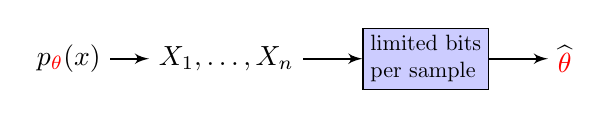
\begin{tikzpicture}[>= latex', node distance = 2cm]
\node at (0,0) (p_th) {$p_{\thetac}(x)$};
\node[right of = p_th] (sample) {$X_1,\ldots,X_n$};
\node[box, right = .75cm of sample, align = left](pm) {limited bits \\ per sample
};
\node[right = .75 cm of pm](th_hat) {$\widehat{\thetac}$};
%\node[below = .1cm of  Xhat]{\textcolor{blue}{reconstruction}};
\draw[->, thick] (p_th) -- (sample);
\draw[->, thick] (sample) -- (pm);
\draw[->, thick] (pm) -- (th_hat);
\end{tikzpicture}
\end{center}
\pause
Estimation error is due to:
\begin{itemize}
\item[(i)] limited data 
\item[(ii)] limited bits
\end{itemize}
\bigskip
\pause
Relevant scenarios:
\begin{itemize}
\pause
\item big data
\pause
\item low-power sensors 
\pause
\item distributed computing / optimization % (bottleneck is due to communication between processing units)

\end{itemize}

\end{frame}

\begin{frame}
\frametitle{This talk: }
\framesubtitle{}
Estimating the mean $\thetac$ of a normal distribution $\mathcal N(\thetac,\sigma^2)$ from one-bit per sample ($\sigma$ is known)
\bigskip

\end{frame}
%

\begin{frame}
\frametitle{Three Encoding Scenarios}

\begin{center}
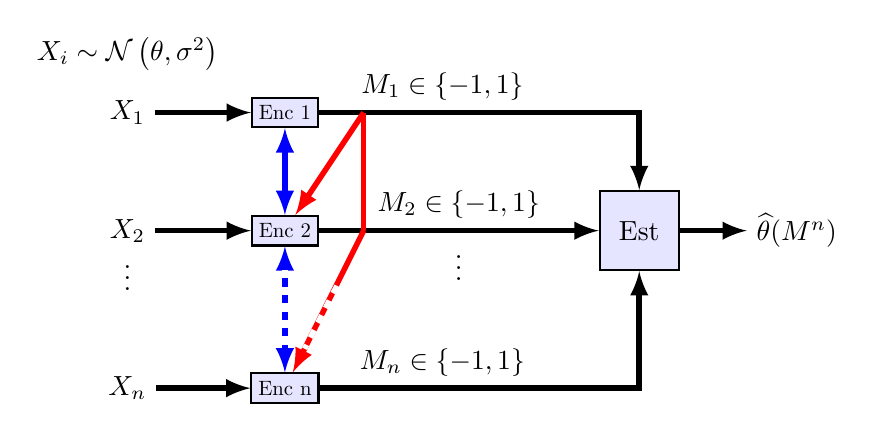
\begin{tikzpicture}[node distance=2cm,auto,>=latex]
  \node at (0,0) (source) {$X_1$} ;
  \node[int1, right of = source, node distance = 2cm, scale = 0.75] (enc1) {Enc 1};  
\draw[->,line width = 2pt] (source) -- (enc1); 

 \node[below of = source, node distance = 1.5cm] (source2) {$X_2$};
\node[int1, right of = source2, node distance = 2cm, scale = 0.75] (enc2) {Enc 2};  
\draw[->,line width = 2pt] (source2) -- (enc2); 

\node[below of = source2, node distance = 2cm] (source3) {$X_n$};
\node[int1, right of = source3, node distance = 2cm, scale = 0.75] (enc3) {Enc n};  
\draw[->,line width = 2pt] (source3) -- (enc3); 

\node[above of = source, node distance = 0.75cm] (dist) {$X_i \sim {\mathcal N} \left(\theta, \sigma^2 \right)$};

\node[Est, right of = enc2, node distance = 4.5cm] (est) {Est};
\draw[->,line width = 2pt] (enc1) -| node[above, xshift = -2.5cm] (mes1) {$M_1 \in \left\{-1,1\right\}$} (est);   
\draw[->,line width = 2pt] (enc2) -- node[above, xshift = 0cm] (mes2) {$M_2 \in \left\{-1,1\right\}$} (est);   
\draw[->,line width = 2pt] (enc3) -| node[above, xshift = -2.5cm]  {$M_n \in \left\{-1,1\right\}$} (est);   
\node[right of = est, node distance = 2cm] (dest) {$\widehat{\theta}(M^n)$};
\draw[->, line width=2pt] (est) -- (dest);

\node[below of = source2, node distance = 0.5cm] {$\vdots$};
\node[below of = enc2, node distance = 0.5cm] {$\vdots$};
\node[below of = mes2, node distance = 0.7cm] {$\vdots$};

\visible<2>{
\draw[<->,line width = 2pt, color = blue] (enc1) -- (enc2);   
\draw[<->,line width = 2pt, color = blue] (enc2) -- (enc3);
\draw[dashed,line width = 2pt, color = white] (enc2)+(0,-0.5) -- +(0,-1.5);}

\visible<3->{
\draw[->,line width = 2pt, color = red] (enc1)+(1,0) -- (enc2);   
\draw[->,line width = 2pt, color = red] (enc2)+(1,0) -- (enc3);
\draw[line width = 2pt, color = red] (enc1)+(1,0) -- +(1,-1.5);

\draw[dashed,line width = 2pt, color = white] (enc2)+(0.66,-0.7) -- +(0.25,-1.5);}

\end{tikzpicture}
\end{center}

\begin{itemize}
\item Distributed: $M_i = f_i(X_i)$
\visible<2->{
\item {\color{blue} Centralized}: $M^n = (M_1,\ldots,M_n) = f(X_1,\ldots,X_n)$ }
\visible<3->{
\item {\color{red} Adaptive / Sequential}: $M_i = f_i(X_i,M^{i-1})$ }
\end{itemize}
\end{frame}

\begin{frame}
\frametitle{Related Work}
\begin{itemize} 
\pause
\item Estimation via compressed information [Han '87], [Zhang \& Berger '88] (centralized)
\pause
\item Estimation from multiple machines subject to a bit constraint [Zhang, Duchi, Jordan, Wainwright '13] (distributed / adaptive)
\pause
\item Distributed hypothesis testing under quantization [Tsitsiklis '88] (distributed)
\pause
\item Remote multiterminal source coding (CEO) [Berger, Zhang, Wiswanathan '96], [Oohama '97] (distributed)
\end{itemize}
\end{frame}

\begin{frame}
\frametitle{Consistency}
Q: in what setting consistent estimation is possible? \\
\bigskip
\pause
A: all ! 
\pause
\bigskip
\textbf{Proof:}
\[
M_i = \mathbf 1(X_i>0),\quad i=1,\ldots,n
\]
(distributed setting)
\pause
\[
\frac{1}{n}\sum_{i=1}^n M_i \rightarrow \Prob\left(X>0 \right) = \Phi\left(\thetac / \sigma \right)
\]
\end{frame}

%SAY: supper slow, of course. Can we do better? what is the best possible? 

\subsection{Preliminary}

\begin{frame}
\frametitle{Efficiency}
\textbf{Definition:} \emph{asymptotic relative efficiency (ARE)}:
\[
\mathrm{ARE}(\widehat{\theta}_n) \triangleq \lim_{n\rightarrow \infty} \mathbb E \left[ \left(\widehat{\theta}_n-\theta \right)^2 \right] / \left(\sigma^2 / n \right)
\]
(relative to minimax risk without bit constraint)
%SAY: many definitions for ARE are possible, we use this one becasue our results apply to all of them
\bigskip

\pause
\begin{prop} ARE under centralized encoding is $1$
\end{prop}
\pause
\textbf{Proof:}
\[
\mathbb E \left( \theta- \widehat{\theta} \right)^2 = \overbrace{\mathbb E \left( \theta- \bar{\theta} \right)^2}^{\sigma^2/n} + \underbrace{\mathbb E \left( \bar{\theta}- \widehat{\theta} \right)^2}_{O(2^{-2n})}
\]

\end{frame}

%\begin{frame}
%\frametitle{ARE under Centralized Encoding}
%
%\begin{prop} ARE under centralized encoding is $1$
%\end{prop}
%\pause
%
%\textbf{Proof:}
%\[
%\mathbb E \left( \theta- \widehat{\theta} \right)^2 = \overbrace{\mathbb E \left( \theta- \bar{\theta} \right)^2}^{\sigma^2/n} + \underbrace{\mathbb E \left( \bar{\theta}- \widehat{\theta} \right)^2}_{O(2^{-2n})}
%\]
%\pause
%\begin{itemize}
%\item Encoder is required to describe $\bar{\theta}$ using $n$ bits
%\begin{itemize}
%\item divide parameter space $\Theta$ into $2^n$ regions of equal size
%\item send region index where $\bar{\theta}$ falls
%\end{itemize}
%\end{itemize}
%\bigskip
%\pause
%Note: mean of $\bar{\theta}$ is unknown -- hard to derive a globally optimal strategy
%%SAY: exploration -- exploitation even in this simple setting
%\end{frame}

\begin{frame}
\frametitle{Relation to CEO}

\begin{center}
\vspace{-20pt}
\begin{tikzpicture}[node distance=2cm,auto,>=latex]
  \node at (0,0) (source) {$\thetac_j$} ;
  \node[ssum, right of = source, scale = 0.75] (sum1) {+};
  \node[above of = sum1, node distance = 1cm] (z1) {$Z_{1}$};
  \node[right of  = z1, node distance = 4cm]  {
 $Z_i  \overset{\mathrm{i.i.d}}{\sim}\mathcal N(0,\sigma^2)$ };
  \node[int1, right of = sum1, node distance = 2cm, scale = 0.75] (enc1) {Enc 1};  
\draw[->,line width = 2pt] (source) -- (sum1); 
\draw[->,line width = 2pt] (sum1) -- node[above] {$X_{1}$} (enc1); 
\draw[->,line width = 2pt] (z1) -- (sum1); 

\node[below of = sum1, node distance = 0.5cm] (vdts) {$\vdots$};
\node[below of = enc1, node distance = 0.5cm] (vdts2) {$\vdots$};

 \node[coordinate,below of = source, node distance = 2.5cm] (source2) {};
 \node[ssum, right of = source2, scale = 0.75] (sum2) {+};
  \node[above of = sum2, node distance = 1.2cm] (z2) {$Z_{n}$};
\node[int1, right of = sum2, node distance = 2cm, scale = 0.75] (enc2) {Enc n};  

\node[Est, right of = enc2, node distance = 5cm, yshift = 1cm] (est) {Est};

\draw[->,line width = 2pt] (source) -- (sum2); 
%\draw[->,line width = 1pt, dashed] (source) -- (vdts);
%\draw[->,line width = 1pt, dashed] (vdts)--(vdts2);
%\draw[->,line width = 1pt, dashed] (vdts2) -- (est);

\draw[->,line width = 2pt] (sum2) -- node[above] {$X_{n}$} (enc2); 
\draw[->,line width = 2pt] (z2) -- (sum2); 

%\draw[fill=blue!10] (enc1)+(5,0.5) rectangle (enc2)+(2,-0.5); 

%\node[int1, right of = enc2, node distance = 6cm, scale = 0.75] (est) {Est};
\draw[->,line width = 2pt] (enc1) -- node[above, xshift = 0cm, rotate = -15] (mes1) {one bit} (est);   
\draw[->,line width = 2pt] (enc2) -- node[above, xshift = 0cm, rotate = 12] (mes2) {one bit} (est);   
\node[right of = est, node distance = 1.5cm] (dest) {$\widehat{\thetac}_j$};
\draw[->, line width=2pt] (est) -- (dest);
\end{tikzpicture}
\end{center}
\begin{itemize}
\item $X_{1},\ldots,X_{n} \overset{\mathrm{i.i.d}}{\sim}\mathcal N(\theta,\sigma^2)$
\pause
\item Replicate $k$ times: $\thetac_1,\ldots,\thetac_k \overset{\iid}{\sim} \mathcal N(0,\sigma_0^2)$ 
\pause
\item Block encode $X_{j,1},\ldots,X_{j,n}$ using $k$ bits, $j=1,\ldots,k$
\pause
\item $D_{CEO} = \underset{k,\widehat{\theta}}{\inf} \frac{1}{k} \sum_{j=1}^k \mathbb E \left( \theta_j - \widehat{\theta}_j\right)^2$
\end{itemize}
%SAY: lower bound to our setting
\end{frame}

\begin{frame}
Quadratic Gaussian CEO under optimal rate allocation [Chen, Zhang, Berger, Wicker '04] :
\[
 D_{CEO}  \geq \frac{4}{3} \frac{\sigma^2}{n} + o(1/n) 
\]
%\begin{itemize}
%\item[] CEO distortion satisfies [Chen, Zhang, Berger, Wicker '04]:
%\[ D^\star = \frac{4}{3} %\frac{\sigma^2}{n} + o(n^{-1}) \]
%\end{itemize}
\pause
\begin{alertblock}{Conclusion}
Distributed encoding will hurt you (even if you can repeat experiment and encode over blocks)
\end{alertblock}
\bigskip
%\pause
%\begin{itemize}
%\item In fact [K., Rini, Goldsmith '17]:
%\end{itemize} 
%\[
% D_{CEO} \leq \frac{4}{3} \frac{\sigma^2}{n} + %\frac{\sigma_0^2}{3n} + o(1/n) 
%\]
%(ARE of $4/3$ is achievable with coding over blocks)
%SAY: depending on how large our bound from $k=1$, it tells us that distributed setting is not the limitng factor
\end{frame}

\section{Adaptive Encoding} 
\begin{frame}
\frametitle{Three Encoding Scenarios}

\begin{center}
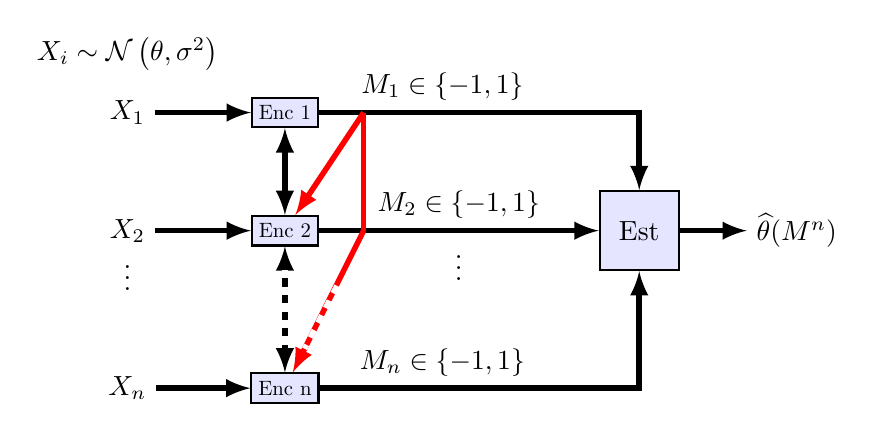
\begin{tikzpicture}[node distance=2cm,auto,>=latex]
  \node at (0,0) (source) {$X_1$} ;
  \node[int1, right of = source, node distance = 2cm, scale = 0.75] (enc1) {Enc 1};  
\draw[->,line width = 2pt] (source) -- (enc1); 

 \node[below of = source, node distance = 1.5cm] (source2) {$X_2$};
\node[int1, right of = source2, node distance = 2cm, scale = 0.75] (enc2) {Enc 2};  
\draw[->,line width = 2pt] (source2) -- (enc2); 

\node[below of = source2, node distance = 2cm] (source3) {$X_n$};
\node[int1, right of = source3, node distance = 2cm, scale = 0.75] (enc3) {Enc n};  
\draw[->,line width = 2pt] (source3) -- (enc3); 

%\node[above of = source3, node distance = 1cm, xshift = -0.5cm] (source3) {$X_i \sim \mathcal N(\theta,\sigma^2)$};

\node[above of = source, node distance = 0.75cm] (dist) {$X_i \sim {\mathcal N} \left(\theta, \sigma^2 \right)$};

\node[Est, right of = enc2, node distance = 4.5cm] (est) {Est};
\draw[->,line width = 2pt] (enc1) -| node[above, xshift = -2.5cm] (mes1) {$M_1 \in \left\{-1,1\right\}$} (est);   
\draw[->,line width = 2pt] (enc2) -- node[above, xshift = 0cm] (mes2) {$M_2 \in \left\{-1,1\right\}$} (est);   
\draw[->,line width = 2pt] (enc3) -| node[above, xshift = -2.5cm]  {$M_n \in \left\{-1,1\right\}$} (est);   
\node[right of = est, node distance = 2cm] (dest) {$\widehat{\theta}(M^n)$};
\draw[->, line width=2pt] (est) -- (dest);

\node[below of = source2, node distance = 0.5cm] {$\vdots$};
\node[below of = enc2, node distance = 0.5cm] {$\vdots$};
\node[below of = mes2, node distance = 0.7cm] {$\vdots$};

\visible<2>{
\draw[<->,line width = 2pt] (enc1) -- (enc2);   
\draw[<->,line width = 2pt] (enc2) -- (enc3);
\draw[dashed,line width = 2pt, color = white] (enc2)+(0,-0.5) -- +(0,-1.5);}

\visible<3->{
\draw[->,line width = 2pt, color = red] (enc1)+(1,0) -- (enc2);   
\draw[->,line width = 2pt, color = red] (enc2)+(1,0) -- (enc3);
\draw[line width = 2pt, color = red] (enc1)+(1,0) -- +(1,-1.5);

\draw[dashed,line width = 2pt, color = white] (enc2)+(0.66,-0.7) -- +(0.25,-1.5);}

\end{tikzpicture}
\end{center}

\begin{itemize}
\item Distributed: $M_i = f_i(X_i)$  \hfill{ARE $\geq 4/3$}
\visible<2->{
\item {Centralized}: $M^n = f(X_1,\ldots,X_n)$ \hfill{ARE $=1$} }
\visible<3->{
\item Next: {\color{red} adaptive / sequential: $M_i = f_i(X_i,M^{i-1})$ \hfill{ARE$=\pi/2$} }  }
\end{itemize}
\end{frame}


\begin{frame}
\frametitle{Main Results (adaptive encoding)}

\begin{theorem}[achievability]
There exists an estimator with ARE $\pi/2$
\end{theorem}

\begin{theorem}[converse]
No estimator have ARE lower than $\pi/2$
\end{theorem}

%\begin{theorem}[one-step optimal strategy]
%The next step one-bit message that minimizes the MSE is of the form $M = \sgn (X-\tau)$ where $\tau$ satisfies the fixed-point equation 
%\[
%\tau = \frac{1}{2} \left( \frac{ \int_{-\infty}^\tau \theta \pi(d\theta) }{\int_{-\infty}^\tau \pi(d\theta)}  + \frac{ \int_{\tau}^\infty \theta \pi(d\theta)}{\int_{\tau}^\infty \pi(d\theta)} \right)
%\]
%\end{theorem}
\end{frame}


\begin{frame}
\frametitle{Achievability}
\framesubtitle{existence of an estimator with ARE $= \pi/2$}

\begin{itemize}
\item[(i)] For $X \sim \mathcal{N}(\theta,\sigma^2)$, $\mathsf{med}(X) = \theta$ 
\pause
\item[(ii)] $\mathsf{med}(X) = \underset{m}{ \mathrm{argmin~}} \mathbb E \left|X-m \right|$
\pause
\item[(iii)] Stochastic gradient descent on $\mathbb E \left| X-\theta \right|$:
\[
\theta_n = \theta_{n-1} + \gamma_n \sgn(X_n - \theta_n)
\]
\[
\widehat{\theta}_n = \frac{1}{n} \sum_{i=1}^n \theta_i 
\]
\end{itemize}
\bigskip
\pause
From [Polyak \& Juditsky '92] (under conditions on $(\gamma_n)$): 
\[
\sqrt{n}(\theta- \widehat{\theta}_n) \rightarrow \mathcal N\left(0, \sigma^2 \pi /2 \right)
\]
(MSE convergence follows from [Polyak '90]) 
\end{frame}
%picture

%\begin{frame}
%\frametitle{Achievability} 
%
%[Polyak \& Juditsky '92]: \\
%
%
%where:
%\begin{itemize}
%\item[(i)] $\gamma_n \rightarrow 0^+$ ``not too slow'' 
%\item[(ii)] $\psi(x) = \mathbb E \varphi(x+Z)$ 
%\item [(iii)] $\chi(x) = \mathbb E \varphi^2(x+Z)$ 
%\item[(iv)] some regularity  conditions on $\varphi$, $\chi$, $\psi$
%\end{itemize}
%Then 
%\[
%\sqrt{n}(\theta- \widehat{\theta}) \rightarrow \mathcal N\left(0,V\right)
%\]
%where $V = \chi(0)/\psi'^2(0)$.  \\
%\medskip
%\pause
%Proof of theorem: take $\varphi(x) = \sgn(x)$
%\end{frame}

\begin{frame}
\frametitle{Converse}
\framesubtitle{ARE $\geq \pi/2$}
Let $\pi(\theta)$ be a prior on $\Theta$. The van-Trees inequality (e.g. [Tsybakov '08]) implies
\[
\mathbb E \left(\theta - \widehat{\theta} \right)^2 \geq \frac{1}{\mathbb E I_\theta(M^n) + I_\pi} \geq \frac{1}{\sum_{i=1}^n I_\theta(M_i|M^{i-1}) + I_\pi} 
\]
$I_\pi$ is the location Fisher information with w.r.t. $\pi(\theta)$ \\

\begin{lem}[K. \& Duchi '17]
\[
I_\theta(M_i|M^{i-1}) \leq \frac{2}{\pi\sigma^2}
\]
\end{lem}
\textbf{Proof}: \\
Stein identity implies that portion maximizing the information is a threshold: $M_i^{-1}(1) = (\theta,\infty)$  \\
The rest follows by induction over number of portions
%SAY: the rest follows by induction over number 
\end{frame}

%\begin{frame}
%\frametitle{One-step Optimal Bit}
%% SAY: previously we bound the inforamtion under any scheme. In addition, it is interesting to understand what is the one-step optimal scheme
%%Q: upon observing $M^{n-1}$, what is the optimal detection region $M_n^{-1}(1)$ that minimizes the MSE ? \\ \pause
%\begin{theorem}
%Let $\pi(\theta)$ be an absolutely continuous log-concave distribution. For $X\sim \mathcal N(\theta,\sigma^2)$ let
%\[
%M = \sgn(X-\tau)
%\]
%where $\tau$ is the unique solution to
%\[
%\tau = \frac{1}{2} \left( \frac{ \int_{-\infty}^\tau \theta \pi(d\theta) }{\int_{-\infty}^\tau \pi(d\theta)}  + \frac{ \int_{\tau}^\infty \theta \pi(d\theta)}{\int_{\tau}^\infty \pi(d\theta)} \right)
%\]
%Then for any $M'(X) \in \{-1,1\}$ and $\widehat{\theta}(M')$:
%\[
%\mathbb E \left(\theta- \widehat{\theta}(M') \right)^2 \geq \mathbb E \left(\theta - \mathbb E[\theta|M] \right)^2
%\]
%\end{theorem}
%\vspace{-20pt}
%\pause
%\begin{alertblock}{Interpertation:}
%\begin{itemize}
%\item One-bit message that minimizes MSE is a threshold detector
%\pause
%\item Leads to a Bayes procedure $\mathbb E \left[\theta | M\right]$
%\end{itemize}
%\end{alertblock}
%
%%SAY: we don't know if this procedure is optimal, what we conjecture that it is
%\end{frame}


%\begin{frame}
%\frametitle{One-step Optimal Scheme}
%Initialization: $P_0(t) = \pi(\theta)$ \\
%Repeat for $n \geq 1$:
%\begin{itemize}
%\item[(i)] $P_n(t) = \Prob(\theta = t|M^n) = \alpha_n P_{n-1}(t) \Phi \left(M_n \frac{t-\tau_{n-1}}{\sigma} \right)$ 
%\item[(ii)] $\widehat{\theta} = \mathbb E[\theta | M^n] = \int t P_n(t)dt $ 
%\item[(iii)] Find $\tau_n$ from 
%\[
%\tau_n = \frac{1}{2} \left( \frac{ \int_{-\infty}^\tau t P_n(t)dt }{\int_{-\infty}^\tau P_n(t)dt}  + \frac{ \int_{\tau}^\infty t P_n(t)dt}{\int_{\tau}^\infty P_n(t)dt} \right)
%\]
%\item[(iv)] $M_{n+1} = \sgn(X_{n+1}-\tau_n)$
%\end{itemize}
%\end{frame}

%\begin{frame}
%\frametitle{Numerical Example}
%\begin{center}
%Normalized empirical risk versus number of samples $n$ \\
%(1000 Monte Carlo experiments)
%\begin{tikzpicture}
%\node at (0,0) {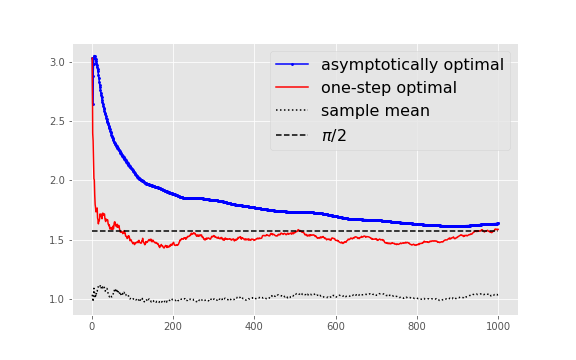
\includegraphics[scale=0.5]{one_bit_adaptive}};
%%\node[color = blue,  minimum width=1cm, align = left] at (1.5,1.5) {assymptotically optimal \eqref{eq:sgd_est}};
%%\node[color = red, minimum width=1cm, align = left] at (1.5,0.55) {one-step optimal \eqref{eq:message_update}} ;
%\node[rotate = 90, scale = 1] at (-5,0) {$n \mathbb E \left(\widehat{\theta}_n - \theta \right)^2$};
%\node[scale = 1] at (0,-3) {$n$};
%%\draw[dashed] (-3.5,1.18) node[left, scale = 0.7] {$\frac{\pi}{2}$}-- (-3,1.18);
%\end{tikzpicture}
%$\theta \sim \unif(-3,3)$
%\end{center}
%\end{frame}

\section{Distributed Encoding}

\begin{frame}
\frametitle{Distributed Encoding}
\framesubtitle{Threshold Detection}
We consider only messages of the form
\[
M_i = \sgn(X_i - t_i),\quad i=1,\ldots,n
\]
\begin{center}
\pause
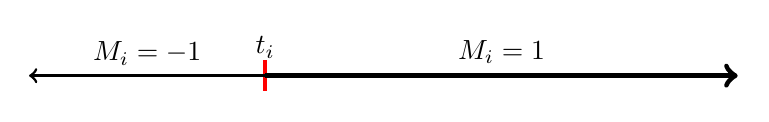
\begin{tikzpicture}
\node[coordinate] at(0,0) (ti) {};
\draw[color = red, line width = 1.5pt] (ti)+(0,0.2) -- node[above, yshift = 0.08cm] {\color{black} $t_i$} +(0,-0.2);
\draw[<-,line width = 1pt] (-3,0) -- node[above] {$M_i=-1$} (ti);
\draw[->,line width = 2pt] (ti) -- node[above] {$M_i=1$} (6,0);
\end{tikzpicture}
\end{center}
Assume:
\[
\lambda_n([a,b]) = \frac{1}{n} \mathsf{card}\left( [a,b]  \cap \left\{t_i \right\} \right)
\]
converges weakly to a probability distribution $\lambda$
\\
\bigskip
\pause
\textbf{Example:} $t_1,\ldots,t_n$ drawn i.i.d. from a distribution $\lambda$ on $\mathbb R$ 

\end{frame}

\begin{frame}
\frametitle{Main Results (distributed encoding)}

\begin{theorem}
\begin{itemize}
\item[(i)] The Maximum likelihood estimator $\widehat{\theta}_{ML}$  satisfies
\[
\sqrt{n}(\theta - \widehat{\theta}_{ML}) \rightarrow \mathcal N\left(0,\sigma^2/K_\lambda(\theta) \right)
\]
where:
\begin{align*}
K_\lambda(\theta) & = \int_{\mathbb R} \eta\left( \frac{t-\theta}{\sigma}\right) \lambda(dt) \\
\eta(x) & = \frac{\phi^2(x)}{\Phi(x)\Phi(-x)}
\end{align*}
% The weight function in the probit analysis
\pause
\item[(ii)] For any estimator $\widehat{\theta}(M_1,\ldots,M_n)$:
\[
\liminf_{c\rightarrow \infty}\, \liminf_{n\rightarrow \infty} \sup_{\tau\,:\,| \tau - \theta| \leq \frac{c}{\sqrt{n}} }  n \mathbb E \left(\widehat{\theta} - \tau \right)^2 \geq \sigma^2/K_\lambda(\theta),
\]

\end{itemize}
\end{theorem}
%{\color{blue} Proof:} $P(M^n|\theta)$ is LAN
\end{frame}


\begin{frame}
\frametitle{Interpretations}
\begin{itemize}
\pause
\item MLE is local asymptotically minimax 
\pause
\item ARE of MLE is $1/K_{\lambda}(\theta)$ -- 
only depends on asymptotic threshold density $\lambda$
\pause
\item  
\[
\mathrm{ARE} = \frac{1}{K_{\lambda}(\theta)}  = \frac{\sigma^2}{\int \eta \left( \frac{t-\theta}{\sigma}\right) \lambda(dt)}
> \pi / 2
\]
(equality iff $\lambda = \delta_{\theta}$)
%SAY: cannot be as good as sequential thresholds
%\item Threshold density $\lambda$ that maximizes
\pause
\item Minimax $\lambda$ can be found using a convex program -- minimax ARE  depends on radius of $\Theta$
%ARE depends on size of parameter space $\Theta$ 
%\begin{center}
%\begin{tikzpicture}
%\node at (0,0)  {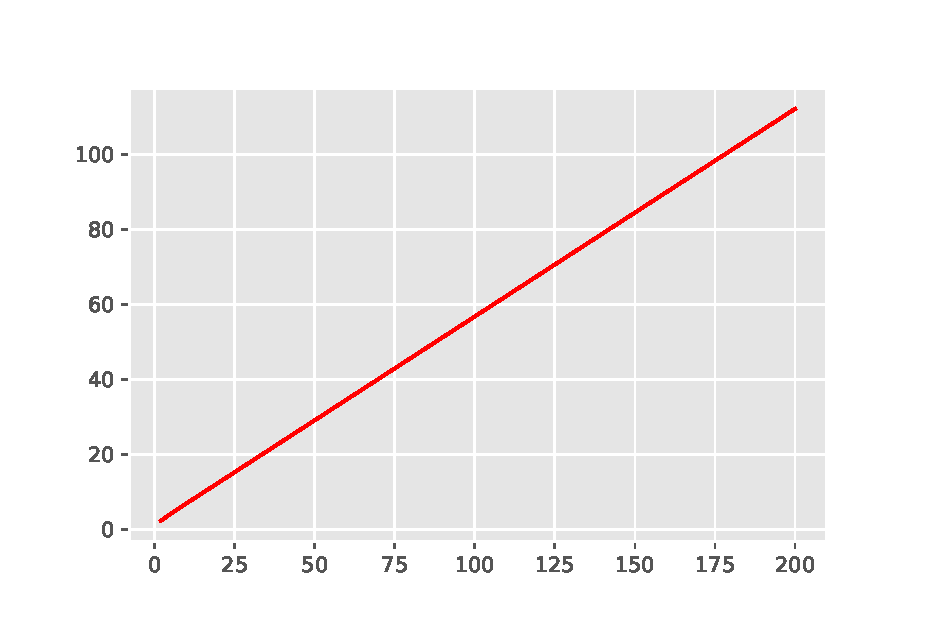
\includegraphics[scale=0.3]{k_vs_b2}};
%\node at (0,-1.7) {$r$};
%\node[rotate = 90] at (-2.3,0) {$1/K_{\lambda^\star}$};
%\end{tikzpicture}
%
%Minimax ARE vs radius $r$ of parameter space
%\end{center}

\end{itemize}

\end{frame}



\section{Summary}

\begin{frame}
\frametitle{Summary}
\begin{itemize}
\pause
\item Centralized encoding: ARE$=1$
\pause
\item Adaptive:
\begin{itemize}
\item ARE is $\pi/2$ (regardless of radius of $\Theta$)
\pause
\item $\sim 1.57$ more samples are required due to 1-bit constraints
\end{itemize}
\pause
%\pause
%\item One-step optimal one-bit message is a threshold detector
\bigskip
\item Distributed threshold detection:
\begin{itemize}
\item ARE of MLE characterized by density of threshold values 
\pause
\item MLE is local asymptotically optimal 
\pause
\item minimax ARE depends on radius of $\Theta$
\end{itemize}
%\item Minimax ARE of MLE depends on size of parameter space
\end{itemize}

\bigskip
\pause
\begin{alertblock}{Open question}
Is there a distributed encoding scheme with ARE that is both finite and independent of radius of $\Theta$ ?
\end{alertblock}

\end{frame}



\begin{frame}
\frametitle{Minimax threshold density}

Minimax $\lambda$ for $\theta \in (-b\sigma,b\sigma)$:
\begin{align*}
\mathrm{maximize} \quad &  \inf_{\tau \in (-b,b)} \int \eta(t-\tau) \lambda(dt)
\\ \nonumber
\mathrm{subject~to} 
\quad & \lambda(dt)\geq 0,\quad \int \lambda(dt) \leq 1. 
\end{align*}

\end{frame}

\begin{frame}
\frametitle{Minimax $\lambda$}
\begin{center}
support of optimal threshold density $\lambda^\star$
\vspace{10pt}
\hspace{-27pt}
\begin{tikzpicture}
\node[int] (b1) at (0,0)  {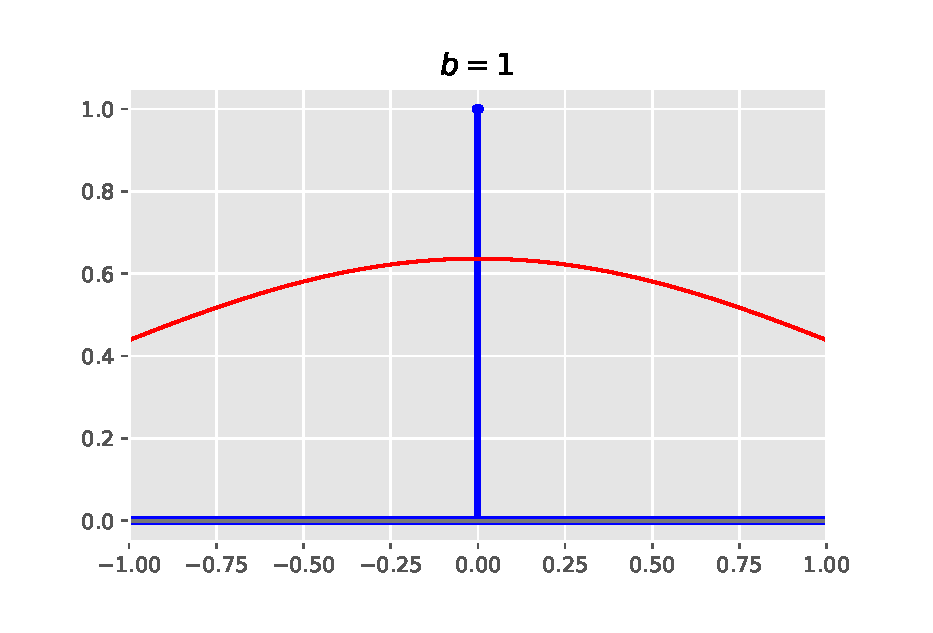
\includegraphics[scale=0.23]{minimax_b_only1}};
\node[int] (b2) at (3.9,0)  {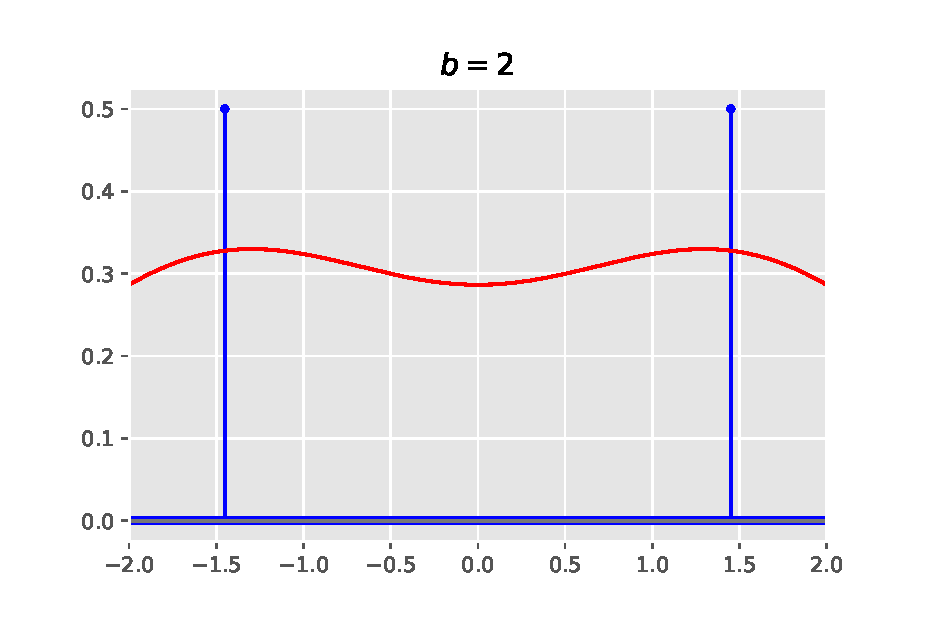
\includegraphics[scale=0.23]{minimax_b_only2}};
\node[int] (b3) at (7.8,0)  {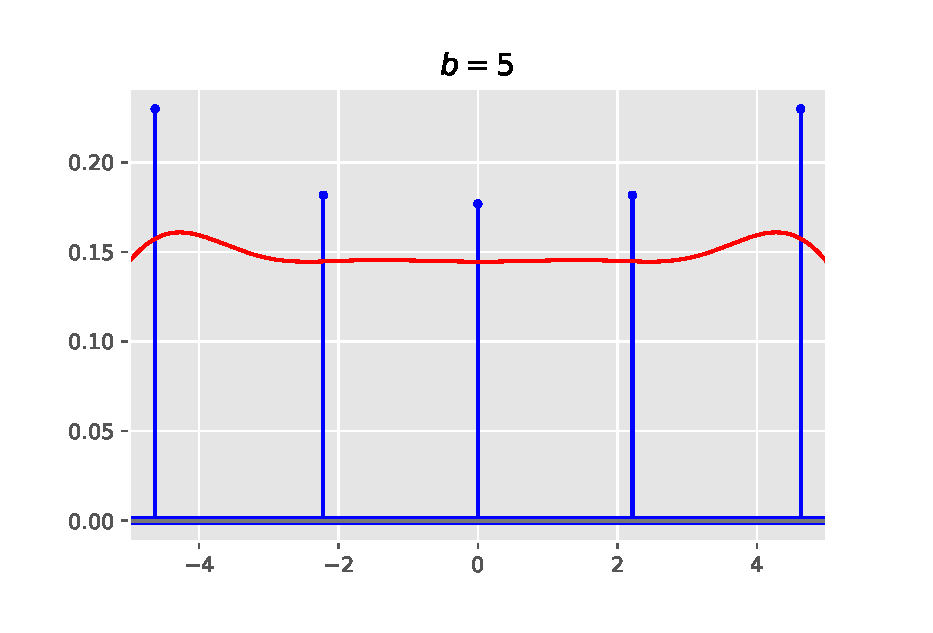
\includegraphics[scale=0.23]{minimax_b_only5}};
\node[int] (b4) at (0,-3)  {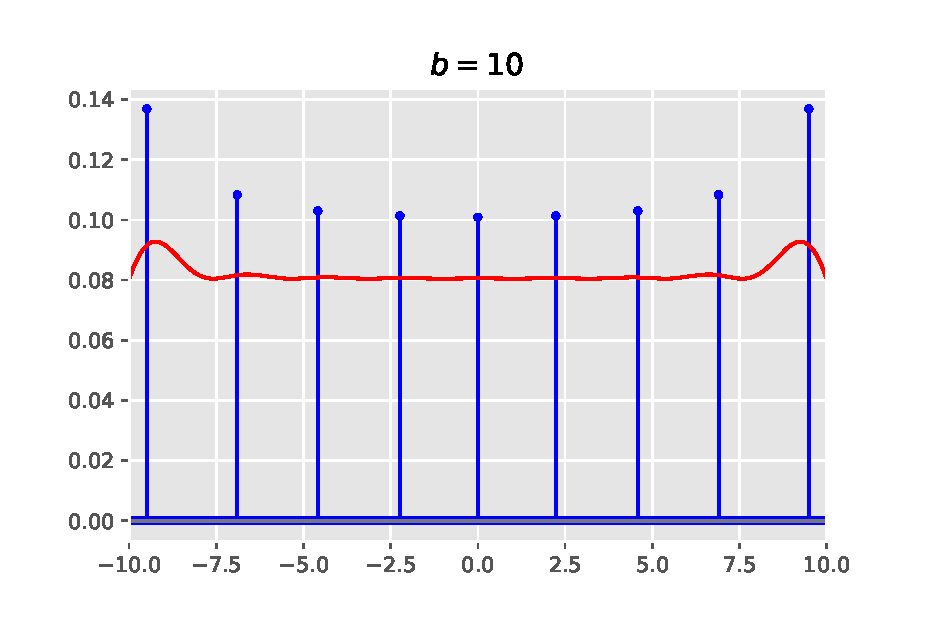
\includegraphics[scale=0.23]{minimax_b_only10}};
\node[int] (b5) at (3.9,-3)  {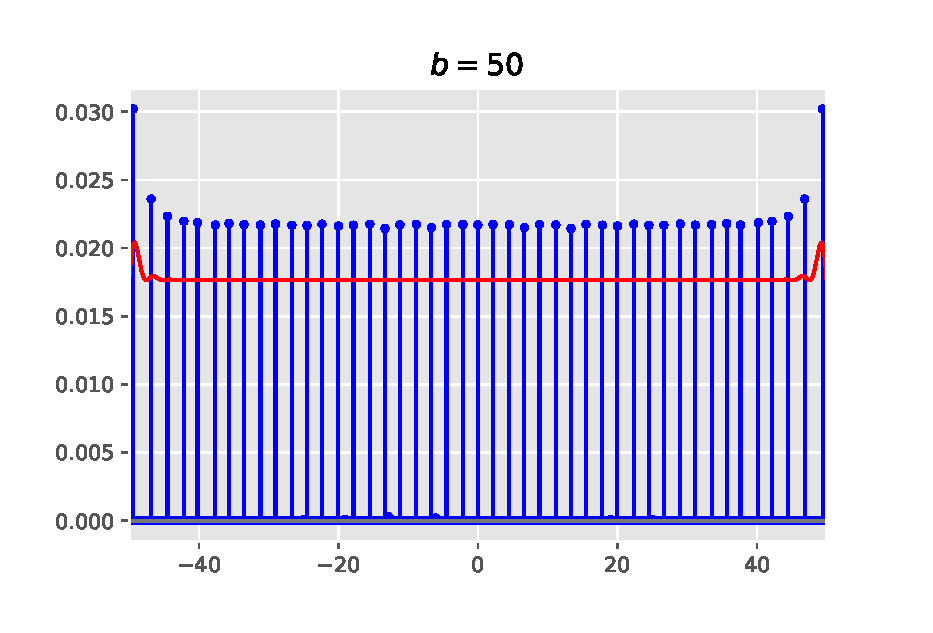
\includegraphics[scale=0.23]{minimax_b_only50}}; 
\node[int] (b6) at (7.8,-3)  {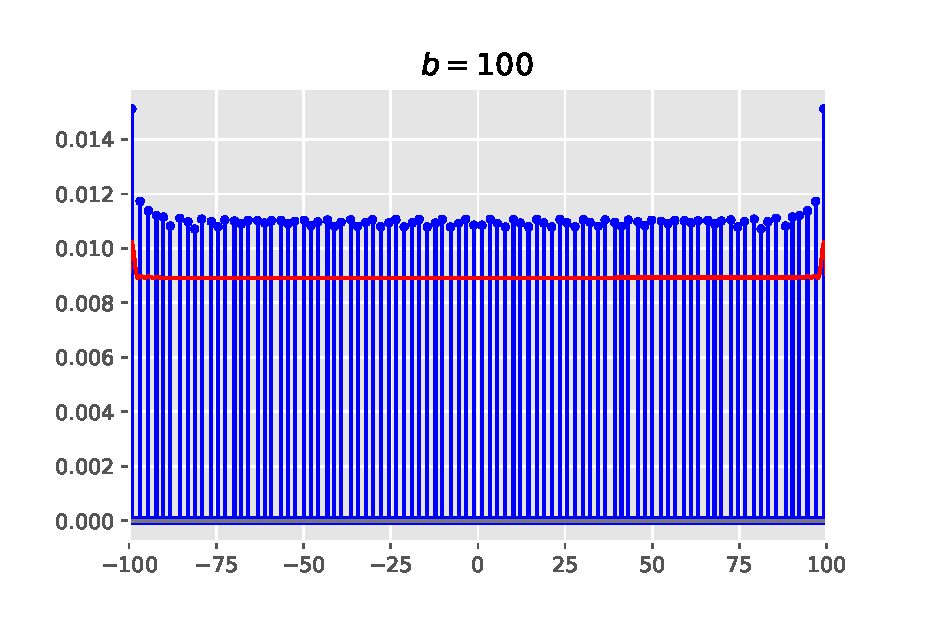
\includegraphics[scale=0.23]{minimax_b_only100}}; 
\end{tikzpicture}
\end{center}
\[
K^\star = \inf_{\theta} K^\star(\theta) = \inf_\theta \int \eta(t-\theta) \lambda^\star(dt)
\]
\end{frame}

\begin{frame}
\frametitle{Minimax $\lambda$}
\begin{center}
Minimax ARE vs size of parameter space %$\Theta= (-\sigma b, \sigma,b)$

\begin{tikzpicture}
\node at (-6,0)  {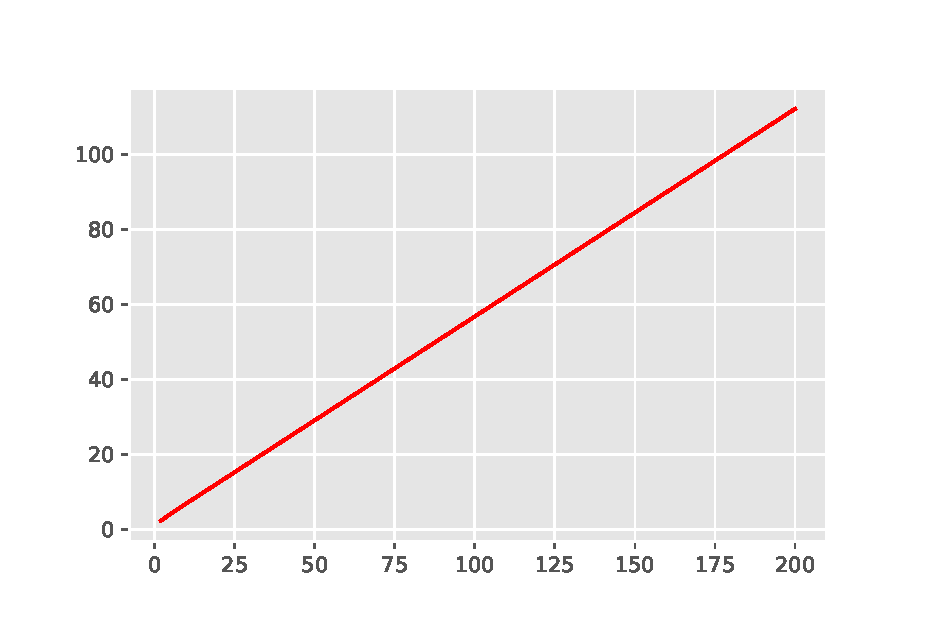
\includegraphics[scale=0.35]{k_vs_b2}};
\node at (0,-2) {$2b$};
\node[rotate = 90] at (-8.5,0) {$1/K^\star$};
\node at (-6,-2) {$2b$};

\node at (0,0)  {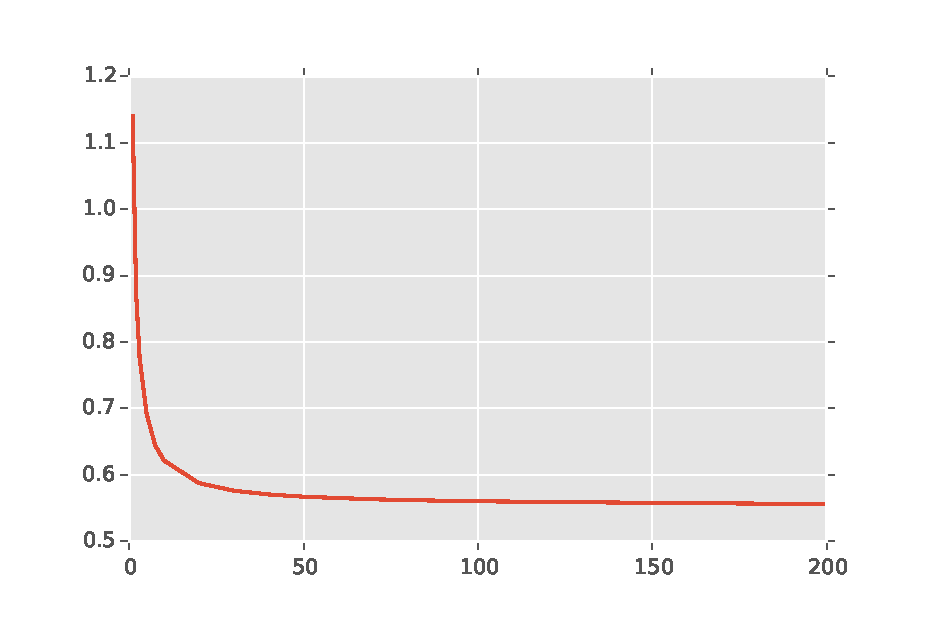
\includegraphics[scale=0.35]{K_vs_b}};
\node at (0,-2) {$2b$};
\node[rotate = 90] at (-2.7,0) {$\frac{1}{2b} \times 1/K^\star$};
\end{tikzpicture}
\end{center}
\begin{itemize}
\item ARE increases with size of parameter space
\end{itemize}

\end{frame}


\begin{frame}
\frametitle{One-step Optimal Scheme}
Initialization: $P_0(t) = \pi(\theta)$ \\
Repeat for $n \geq 1$:
\begin{itemize}
\item[(i)] $P_n(t) = \Prob(\theta = t|M^n) = \alpha_n P_{n-1}(t) \Phi \left(M_n \frac{t-\tau_{n-1}}{\sigma} \right)$ 
\item[(ii)] $\widehat{\theta} = \mathbb E[\theta | M^n] = \int t P_n(t)dt $ 
\item[(iii)] Find $\tau_n$ from 
\[
\tau_n = \frac{1}{2} \left( \frac{ \int_{-\infty}^\tau t P_n(t)dt }{\int_{-\infty}^\tau P_n(t)dt}  + \frac{ \int_{\tau}^\infty t P_n(t)dt}{\int_{\tau}^\infty P_n(t)dt} \right)
\]
\item[(iv)] $M_{n+1} = \sgn(X_{n+1}-\tau_n)$
\end{itemize}
\end{frame}

\begin{frame}
\frametitle{Numerical Example}
\begin{center}
Normalized empirical risk versus number of samples $n$ \\
(1000 Monte Carlo experiments)
\begin{tikzpicture}
\node at (0,0) {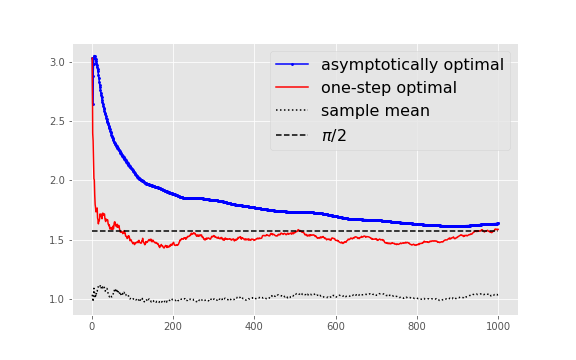
\includegraphics[scale=0.5]{one_bit_adaptive}};
%\node[color = blue,  minimum width=1cm, align = left] at (1.5,1.5) {assymptotically optimal \eqref{eq:sgd_est}};
%\node[color = red, minimum width=1cm, align = left] at (1.5,0.55) {one-step optimal \eqref{eq:message_update}} ;
\node[rotate = 90, scale = 1] at (-5,0) {$n \mathbb E \left(\widehat{\theta}_n - \theta \right)^2$};
\node[scale = 1] at (0,-3) {$n$};
%\draw[dashed] (-3.5,1.18) node[left, scale = 0.7] {$\frac{\pi}{2}$}-- (-3,1.18);
\end{tikzpicture}
$\theta \sim \unif(-3,3)$
\end{center}
\end{frame}


\end{document}